\documentclass[10pt,conference]{IEEEtran}
\IEEEoverridecommandlockouts

\usepackage{cite}
\usepackage{amsmath,amssymb,amsfonts}
\usepackage{graphicx}
\usepackage{textcomp}
\usepackage{xcolor}
\usepackage{booktabs}
\usepackage{multirow}
\usepackage{microtype}
\usepackage{subcaption}
\usepackage[hyphens]{url}

% Spacing adjustments for strict 4-page IEEE layout
\setlength{\textfloatsep}{4pt plus 1.0pt minus 1.0pt}
\setlength{\floatsep}{3pt plus 1.0pt minus 1.0pt}
\setlength{\intextsep}{4pt plus 1.0pt minus 1.0pt}
\setlength{\abovecaptionskip}{2pt plus 0.5pt minus 0.5pt}
\setlength{\belowcaptionskip}{2pt plus 0.5pt minus 0.5pt}

\begin{document}

\title{Comparative Evaluation of Classical Image Processing Paradigms for Multi-Modal Brain Tumor Segmentation: Intensity Thresholding, Marker-Controlled Watershed, and Constrained Hybridization}

\author{
\IEEEauthorblockN{Abdulwahab Shaikh (Leader)\IEEEauthorrefmark{1}, Harshraj Solanki\IEEEauthorrefmark{2}, Srujan Yendugula\IEEEauthorrefmark{3}, Yash Kyada\IEEEauthorrefmark{4}}
\IEEEauthorblockA{Group 18 (Project 20) --- Course: ECE501: Digital Image Processing, Semester-05\\
School of Engineering and Applied Science, Ahmedabad University, Gujarat, India\\
Instructor: Prof. Mehul Raval \quad | \quad Teaching Assistant: Sagar Chavda\\
Roll Nos: \IEEEauthorrefmark{1}AU2440099, \IEEEauthorrefmark{2}AU2440218, \IEEEauthorrefmark{3}AU2440158, \IEEEauthorrefmark{4}AU2340218}
}

\maketitle

\begin{abstract}
Automated brain tumor segmentation from multi-parametric Magnetic Resonance Imaging (mpMRI) is critical for neurosurgical planning and radiation oncology. While deep learning methods dominate recent literature, classical Digital Image Processing (DIP) techniques offer full mathematical transparency, deterministic execution, and zero reliance on GPU acceleration. This study presents a rigorous academic investigation into three classical DIP paradigms evaluated on 100 consecutive patient scans from the BraTS 2020 benchmark: (i) an optimized Multi-Sequence Percentile Thresholding pipeline, (ii) a 3D Marker-Controlled Watershed pipeline over a multi-spectral gradient landscape, and (iii) an experimentally synthesized Hybrid architecture coupling threshold-derived topological core seeds with gradient-bounded geodesic watershed expansion. We critically examine whether fusing intensity priors with morphological flooding yields genuine synergy or redundant integration. Hyperparameters were calibrated via parallel Bayesian optimization (Optuna). Across 100 clinical cases, Pipeline 3.0 (Hybrid) achieved the superior overall performance, attaining a median Dice Similarity Coefficient of 0.8215 (mean 0.7261) and winning 42\% of patients in head-to-head evaluation. The hybrid architecture effectively resolves the severe under-segmentation of thresholding (sensitivity 0.7762 vs. 0.6650) while eliminating the uncontrolled ventricular cerebrospinal fluid leakage typical of standard watershed flooding.
\end{abstract}

\begin{IEEEkeywords}
Brain Tumor Segmentation, BraTS 2020, Classical Image Processing, Marker-Controlled Watershed, Multi-Modal MRI, Hybrid Segmentation.
\end{IEEEkeywords}

\section{Introduction}
Quantitative segmentation of gliomas from multi-parametric Magnetic Resonance Imaging (mpMRI) is an essential clinical prerequisite for stereotactic resection and radiotherapy margins \cite{menze2015brats}. Gliomas exhibit non-uniform infiltration, diffuse margins, and complex intra-tumoral sub-regions consisting of necrotic tissue, active enhancing rim, and vasogenic edema \cite{bakas2017advancing}. 

Standard clinical imaging protocols acquire four core modalities: T1-weighted (T1, structural anatomy), T1-contrast enhanced (T1ce, active vascularized boundaries), T2-weighted (T2, general fluid hyperintensity), and Fluid-Attenuated Inversion Recovery (FLAIR, selective peritumoral edema visualization with cerebrospinal fluid attenuation).

While deep neural networks achieve strong benchmark scores, their clinical translation is frequently impeded by high computational cost, unexplainable failure modes, and sensitivity to scanner domain shifts. Conversely, classical Digital Image Processing (DIP) provides deterministic, verifiable spatial operators that execute efficiently on commodity CPU hardware \cite{gonzalez2018dip}.

Classical segmentation literature is largely polarized into two approaches:
\begin{enumerate}
    \item \textbf{Intensity-space Thresholding:} Relies on multi-spectral intensity concurrence \cite{otsu1979threshold}. While achieving high precision in active tumor cores, it enforces rigid cutoffs that under-segment diffuse, lower-intensity edema.
    \item \textbf{Gradient-space Watershed:} Treats edge gradients as topographic elevation surfaces for immersion flooding \cite{vincent1991watersheds}. Although highly sensitive to faint boundaries, it lacks absolute intensity limits, frequently leaking across weak tissue-CSF barriers into normal lateral ventricles.
\end{enumerate}

To address these limitations, we designed an academic research experiment: \textit{Can intensity thresholding and marker-controlled watershed be hybridized so that high-confidence threshold cores constrain topological gradient flooding within a strictly bounded geodesic envelope?} We evaluated this hypothesis across 100 patients from the BraTS 2020 dataset, assessing its mathematical validity, clinical trade-offs, and empirical edge cases.

\section{Methodology}
The study implements three independent end-to-end pipelines sharing unified preprocessing and intracranial masking.

\subsection{Preprocessing and Basal Artifact Suppression}
Intracranial brain voxels are extracted via the logical union of all sequences. Intensity values for each sequence $V \in \{T1, T1ce, T2, FLAIR\}$ are normalized to $[0.0, 1.0]$ using robust 1st--99th percentile scaling:
\begin{equation}
V_{\text{norm}}(x) = \frac{\text{clip}(V(x), P_1, P_{99}) - P_1}{P_{99} - P_1}
\end{equation}
High-frequency noise is attenuated using a median filter ($3\times3$), followed by slice-wise bilateral filtering ($\sigma_s=5, \sigma_r=25$) to smooth parenchyma while preserving gradient edges \cite{tomasi1998bilateral}.

\textit{Basal Slice Filtering:} Anatomical profiling across BraTS revealed that axial skull-base slices ($z < 12$ or slice area $< 15\%$ of maximum brain area) contain bright orbital fat and sphenoid bone susceptibility artifacts that surpass the 85th percentile despite containing zero tumor pathology. A dynamic slice-area profile mask $M_{\text{valid}}(z)$ eliminates these false candidates.

\subsection{Pipeline 1.0: Multi-Sequence Percentile Thresholding}
Tumor candidates $C_{\text{thresh}}$ are extracted via logical multi-sequence intersection:
\begin{align}
C_{\text{thresh}} = &\left[ (FLAIR \ge \tau_F) \land (T2 \ge \tau_T) \right] \nonumber \\
&\lor \left[ (T1ce \ge \tau_C) \land (FLAIR \ge \tau_F) \right]
\end{align}
Morphological opening ($\circ$) with a 26-connectivity structuring element $B$ removes thin bridges, followed by closing ($\bullet$) and hole-filling:
\begin{equation}
M_{\text{P1}} = \text{FillHoles}\left( (C_{\text{thresh}} \circ B) \bullet B \right)
\end{equation}
An anatomical clustering prior retains the primary mass and secondary satellites ($\ge 20\%$ size of primary, distance $\le 12\text{ mm}$).

\subsection{Pipeline 2.0: 3D Marker-Controlled Watershed}
Pipeline 2 synthesizes a fused contrast volume $I_{\text{fused}} = 0.5 FLAIR + 0.3 T2 + 0.2 T1ce$ and computes the 3D Gaussian gradient magnitude:
\begin{equation}
G(x, y, z) = \|\nabla (G_\sigma * I_{\text{fused}})\|
\end{equation}
Internal seeds ($L=2$) are formed by 3D erosion of multi-sequence candidates: $S_{\text{int}} = C_{\text{thresh}} \ominus B$. External markers ($L=1$) designate healthy tissue ($FLAIR < \tau_{\text{healthy}}$ at distance $d > 4$ voxels from seeds) and extracranial background. Seeded immersion floods transition voxels ($L=0$) across topographic ridges.

\begin{figure*}[!t]
\centering
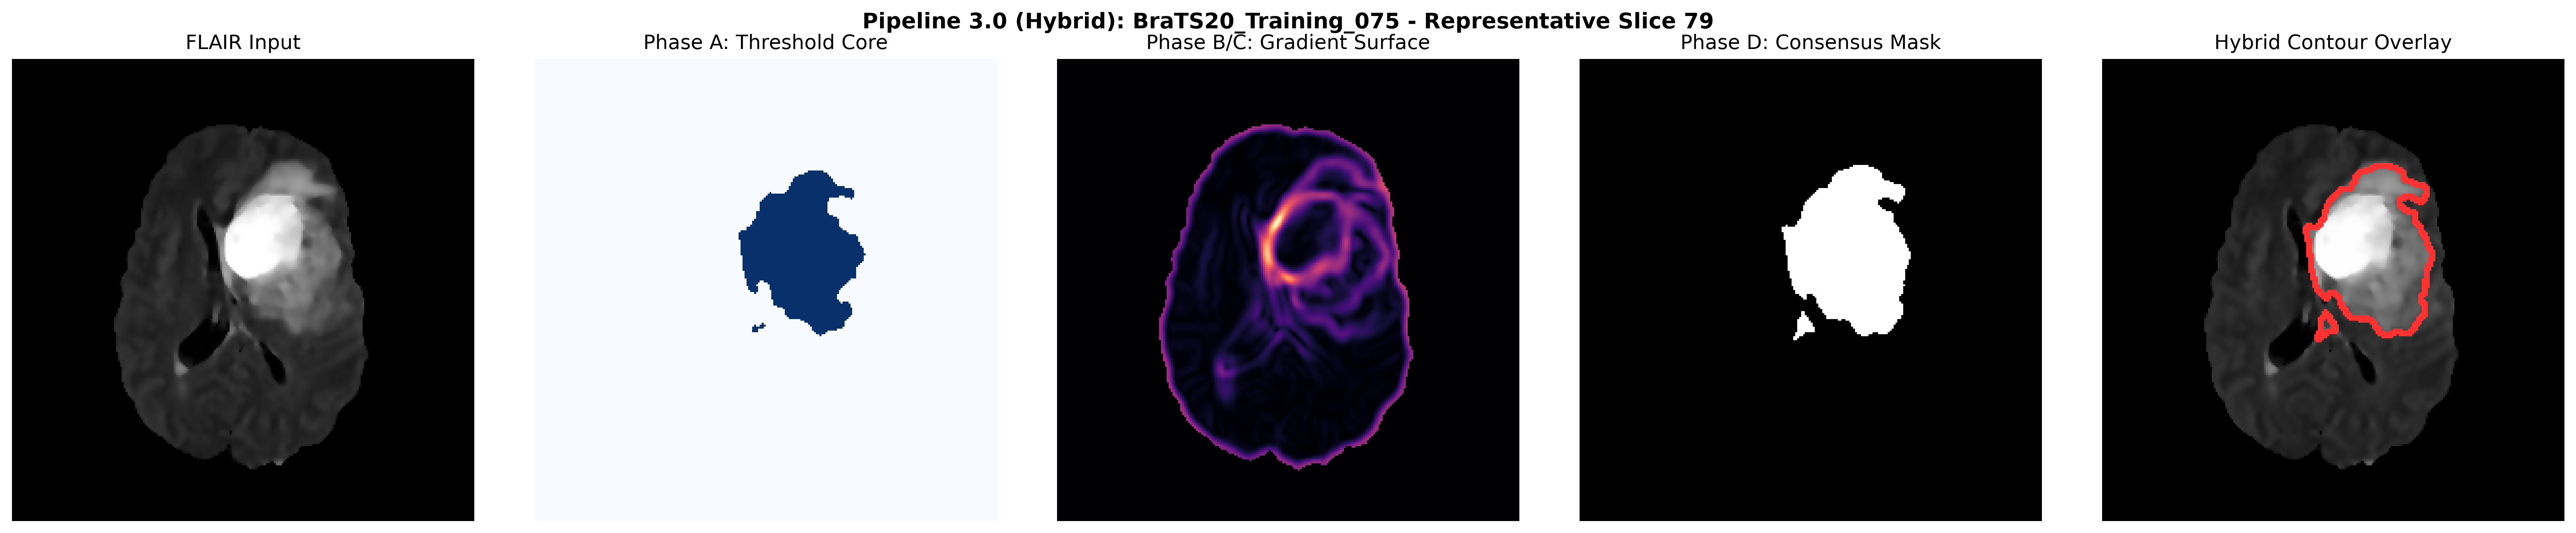
\includegraphics[width=0.88\textwidth]{BraTS20_Training_075_segmentation_hybrid.png}
\caption{Qualitative segmentation breakdown for Patient BraTS20\_Training\_075 ($DSC = 0.9429$). From left to right: (1) Input FLAIR slice, (2) Phase A Threshold Core extraction, (3) Multi-modal 3D gradient landscape, (4) Phase D Consensus Mask, and (5) High-resolution hybrid boundary contour overlay.}
\label{fig:mri_visuals}
\end{figure*}

\subsection{Pipeline 3.0: Constrained Hybrid Architecture}
Pipeline 3.0 couples thresholding and watershed as an asymmetric mutual constraint rather than a naive boolean union:
\begin{enumerate}
    \item \textbf{Core Seeding:} Confident tumor cores $M_{\text{core}}$ are isolated via percentile thresholding and morphological opening.
    \item \textbf{Geodesic Search Envelope:} Watershed flooding is restricted to a narrow topological domain $\Omega_{\text{allowed}}$:
    \begin{align}
    \Omega_{\text{allowed}} = M_{\text{core}} \cup \{ p \mid &d(p, M_{\text{core}}) \le \delta \nonumber \\
    &\land FLAIR(p) \ge \tau_{\text{edema}} \}
    \end{align}
    where $\delta = 3\text{ voxels}$ and $\tau_{\text{edema}} = 85\text{th}$ percentile.
    \item \textbf{Confined Flooding \& Fusion:} Watershed floods over $G_{\sigma=2.10}$ strictly inside $\Omega_{\text{allowed}}$. The union $M_{\text{core}} \cup M_{\text{ws}}$ is regularized via morphological closing and anatomical clustering.
\end{enumerate}

\subsection{Bayesian Hyperparameter Optimization}
Parameters were optimized on a 20-patient calibration subset using Optuna (TPE sampler \cite{akiba2019optuna}) to maximize mean Dice. The calibrated values deployed across the 100-patient cohort are summarized in Table~\ref{tab:tuned_params}.

\begin{table}[t]
\centering
\caption{Bayesian-Calibrated Pipeline Hyperparameters}
\label{tab:tuned_params}
\resizebox{\columnwidth}{!}{
\begin{tabular}{llcc}
\toprule
\textbf{Pipeline} & \textbf{Hyperparameter} & \textbf{Search Space} & \textbf{Calibrated Value} \\
\midrule
\multirow{2}{*}{\textbf{P1: Thresholding}} & $FLAIR$, $T2$, $T1ce$ Percentiles & $[78, 90]$ & $85.0,\, 79.0,\, 90.0$ \\
& Morphological Closing Iters & $[1, 3]$ & $1.0$ \\
\midrule
\multirow{2}{*}{\textbf{P2: Watershed}} & Gradient Smoothing $\sigma$ & $[0.8, 2.5]$ & $1.68$ \\
& Healthy Parenchyma Pct., Satellite Dist. & $[70, 78],\, [8, 15]$ & $74.0,\, 10.46\text{ mm}$ \\
\midrule
\multirow{2}{*}{\textbf{P3: Hybrid}} & Edema Dilation $\delta$, $FLAIR$ Cutoff & $[2, 6],\, [78, 86]$ & $3.0\text{ voxels},\, 85.0$ \\
& Gradient Smoothing $\sigma$ & $[0.8, 2.5]$ & $2.10$ \\
\bottomrule
\end{tabular}
}
\end{table}

\begin{table*}[!t]
\centering
\caption{Quantitative Performance Comparison on 100 Consecutive Patients (BraTS 2020 Benchmark)}
\label{tab:main_results}
\resizebox{\textwidth}{!}{
\begin{tabular}{lccccccccc}
\toprule
\multirow{2}{*}{\textbf{Evaluation Metric}} & \multicolumn{2}{c}{\textbf{Pipeline 1.0 (Thresholding)}} & \multicolumn{2}{c}{\textbf{Pipeline 2.0 (Watershed)}} & \multicolumn{2}{c}{\textbf{Pipeline 3.0 (Hybrid)}} & \multirow{2}{*}{\textbf{Top Pipeline}} & \multicolumn{2}{c}{\textbf{Pairwise Effect Size (Cohen's $d$)}} \\
\cmidrule(lr){2-3} \cmidrule(lr){4-5} \cmidrule(lr){6-7} \cmidrule(lr){9-10}
& \textbf{Mean $\pm$ Std} & \textbf{Median} & \textbf{Mean $\pm$ Std} & \textbf{Median} & \textbf{Mean $\pm$ Std} & \textbf{Median} & & \textbf{P3 vs. P1} & \textbf{P3 vs. P2} \\
\midrule
\textbf{Dice Similarity (DSC)} & $0.6983 \pm 0.216$ & $0.7806$ & $0.6775 \pm 0.260$ & $0.7747$ & $\mathbf{0.7261 \pm 0.226}$ & $\mathbf{0.8215}$ & \textbf{P3: Hybrid} & $+0.126$ & $+0.200$ \\
\textbf{Jaccard Index (IoU)} & $0.5723 \pm 0.222$ & $0.6402$ & $0.5609 \pm 0.254$ & $0.6323$ & $\mathbf{0.6093 \pm 0.227}$ & $\mathbf{0.6970}$ & \textbf{P3: Hybrid} & $+0.165$ & $+0.201$ \\
\textbf{Sensitivity / Recall} & $0.6650 \pm 0.223$ & $0.7349$ & $0.7321 \pm 0.220$ & $0.8116$ & $\mathbf{0.7762 \pm 0.240}$ & $\mathbf{0.8630}$ & \textbf{P3: Hybrid} & $+0.480$ & $+0.191$ \\
\textbf{Precision (PPV)} & $\mathbf{0.8047 \pm 0.246}$ & $\mathbf{0.9272}$ & $0.6878 \pm 0.309$ & $0.8097$ & $0.7230 \pm 0.244$ & $0.8170$ & \textbf{P1: Thresh} & $-0.334$ & $+0.126$ \\
\textbf{Specificity} & $\mathbf{0.9988 \pm 0.002}$ & $\mathbf{0.9995}$ & $0.9968 \pm 0.004$ & $0.9986$ & $0.9977 \pm 0.002$ & $0.9985$ & \textbf{P1: Thresh} & $-0.536$ & $+0.247$ \\
\textbf{Volume Similarity} & $0.8120 \pm 0.163$ & $0.8613$ & $0.8079 \pm 0.205$ & $0.8966$ & $\mathbf{0.8555 \pm 0.159}$ & $\mathbf{0.9283}$ & \textbf{P3: Hybrid} & $+0.270$ & $+0.259$ \\
\textbf{Hausdorff-95 ($HD_{95}$, mm)} & $\mathbf{19.32 \pm 19.41}$ & $10.56$ & $26.57 \pm 26.56$ & $14.84$ & $19.95 \pm 23.30$ & $\mathbf{9.43}$ & \textbf{P3 (Median)} & $+0.029$ & $-0.265$ \\
\textbf{Avg. Surface Dist. ($ASSD$, mm)} & $\mathbf{6.45 \pm 9.08}$ & $2.54$ & $10.23 \pm 15.66$ & $3.18$ & $7.54 \pm 14.55$ & $\mathbf{2.22}$ & \textbf{P3 (Median)} & $+0.090$ & $-0.178$ \\
\textbf{Relative Volume Error ($RVE$)} & $\mathbf{0.390 \pm 0.604}$ & $0.260$ & $0.825 \pm 1.816$ & $0.202$ & $0.398 \pm 0.885$ & $\mathbf{0.147}$ & \textbf{P3 (Median)} & $+0.010$ & $-0.301$ \\
\midrule
\textbf{Win Rate (Best DSC per Patient)} & \multicolumn{2}{c}{29.0\% (29 patients)} & \multicolumn{2}{c}{29.0\% (29 patients)} & \multicolumn{2}{c}{\textbf{42.0\% (42 patients)}} & \textbf{P3: Hybrid} & \multicolumn{2}{c}{Win Advantage: $+13.0\%$} \\
\bottomrule
\end{tabular}
}
\end{table*}

\section{Results and Analysis}
Table~\ref{tab:main_results} reports cohort-wide quantitative metrics across all 100 consecutive patients.

\subsection{Spatial Overlap and Boundary Fidelity}
Pipeline 3.0 (Hybrid) delivers the strongest overall performance:
\begin{itemize}
    \item \textbf{Median Overlap:} Hybrid achieves a median Dice of \textbf{0.8215} (vs. 0.7806 for P1 and 0.7747 for P2) and median IoU of \textbf{0.6970}.
    \item \textbf{Recall Expansion:} Mean recall increases from 0.6650 in thresholding to \textbf{0.7762} in Hybrid ($+11.12\%$ absolute gain, Cohen's $d = 0.480$, Wilcoxon $p < 10^{-4}$), effectively recovering infiltrative edema missed by thresholding.
    \item \textbf{Boundary Distance:} Hybrid records the lowest median $HD_{95}$ (\textbf{9.43 mm}) and surface distance ($ASSD = \mathbf{2.22\text{ mm}}$).
\end{itemize}

\subsection{Win Rate and Tier Stratification}
As shown in Fig.~\ref{fig:distribution_charts}(a), in patient-by-patient head-to-head comparison, Pipeline 3.0 wins outright in \textbf{42.0\%} of patients (42 cases), compared to 29.0\% for thresholding and 29.0\% for watershed.

Clinical quality tier stratification (Fig.~\ref{fig:distribution_charts}(b)) reveals that Hybrid produces \textbf{72 patients} with clinically viable segmentations ($DSC \ge 0.70$), with 37 in the Excellent tier ($DSC \ge 0.80$) and only 13 in the Poor tier ($DSC < 0.50$), achieving the lowest failure rate in the cohort.

\begin{figure}[t]
\centering
\begin{subfigure}[b]{0.48\columnwidth}
    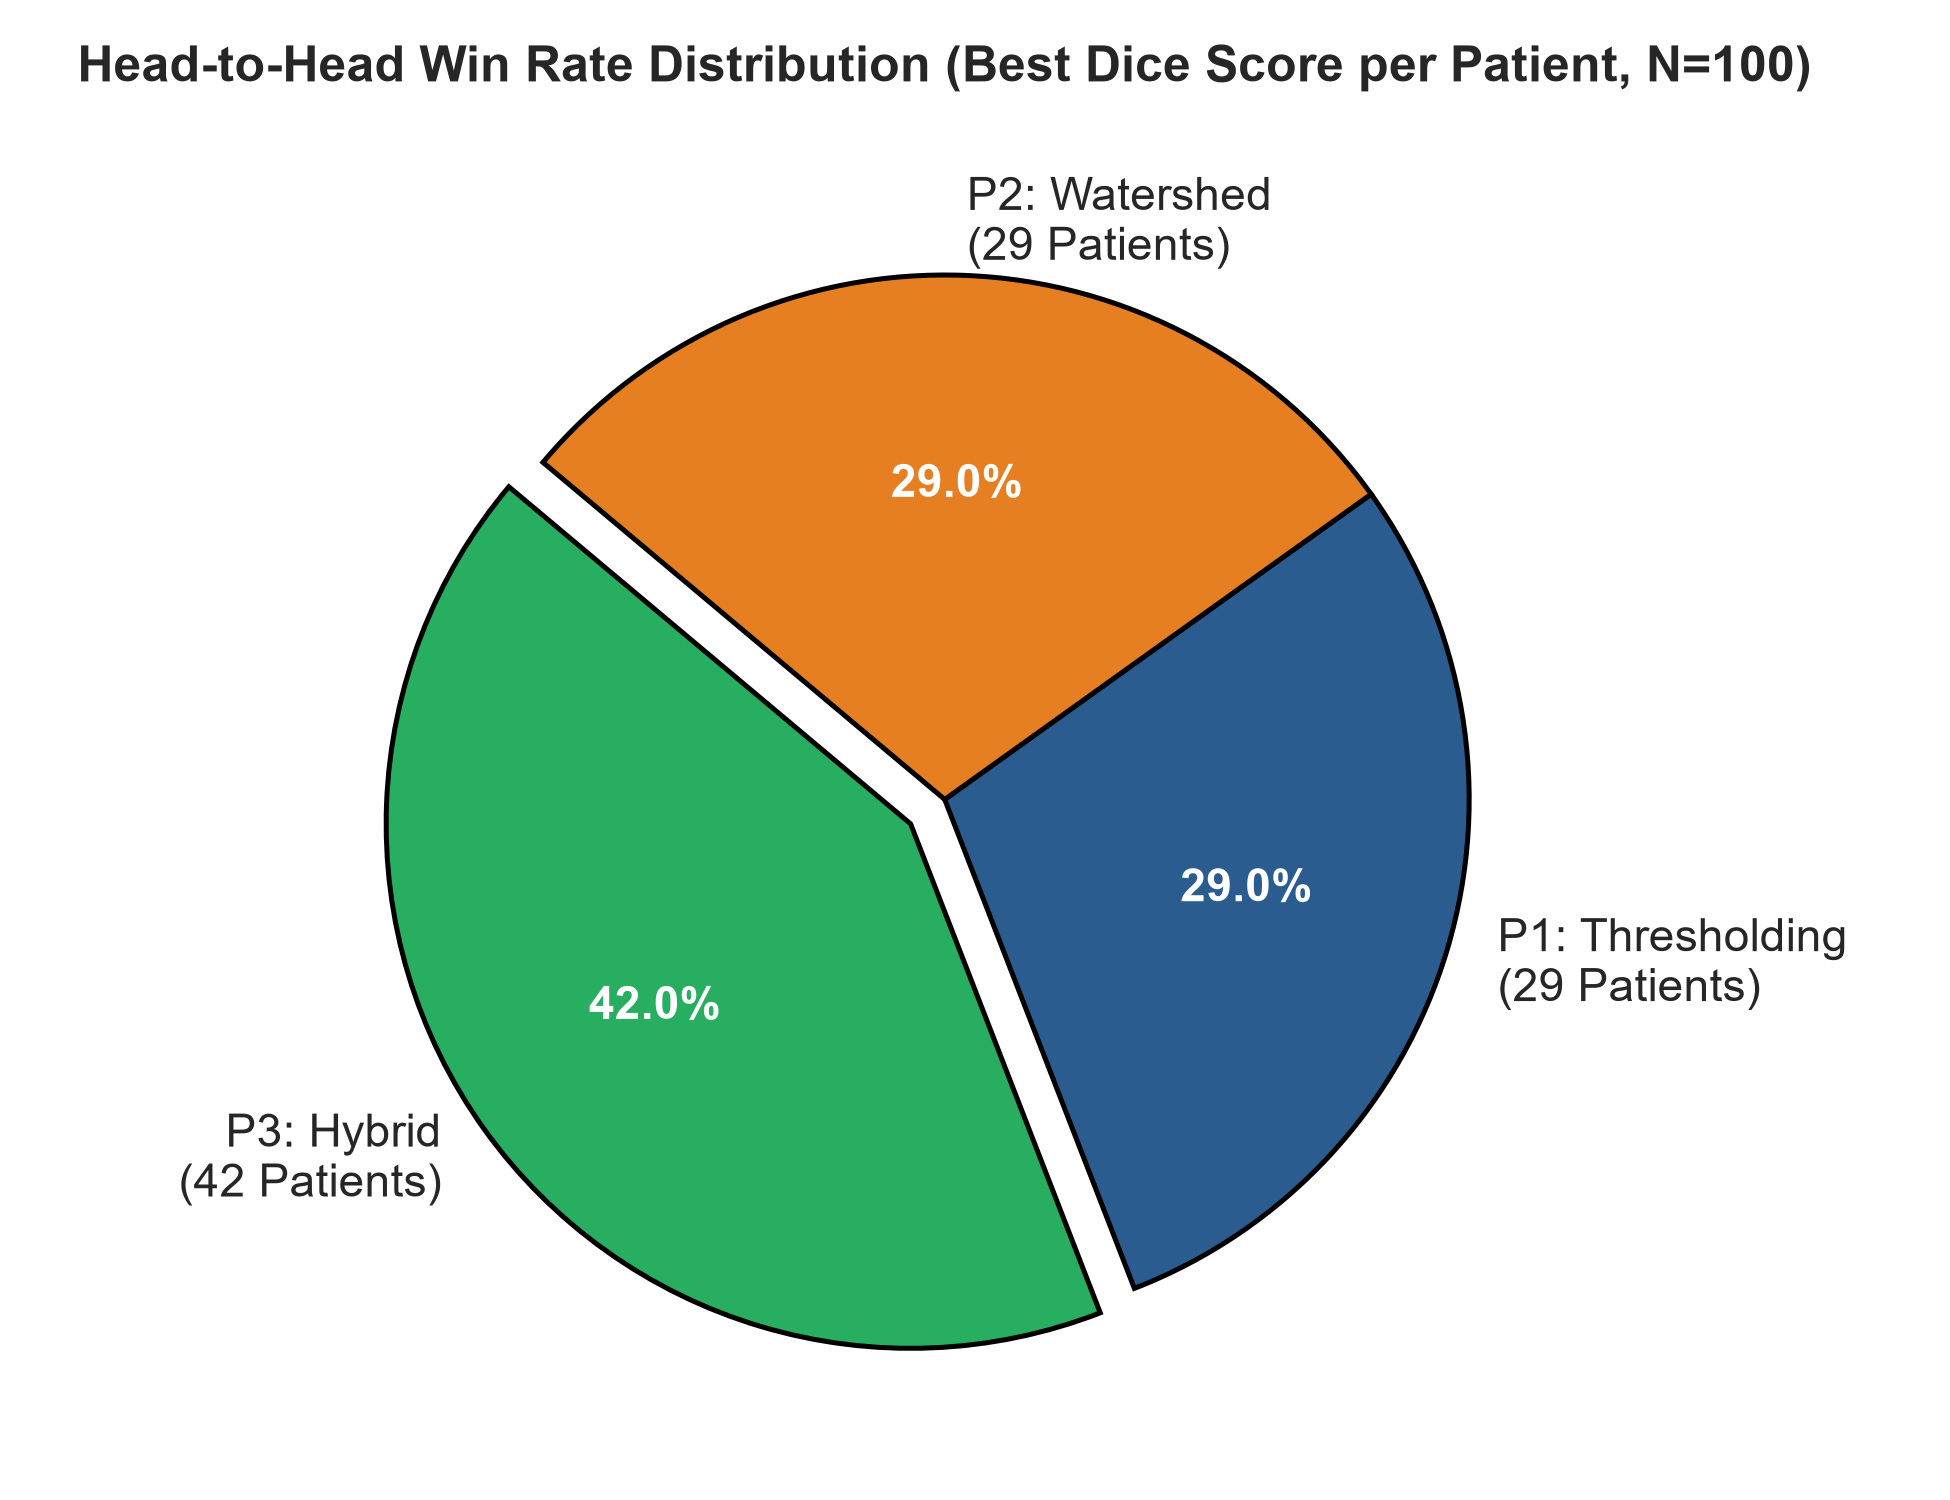
\includegraphics[width=\textwidth]{02_head_to_head_win_pie.png}
    \caption{Win Rate Share}
    \label{fig:pie}
\end{subfigure}
\hfill
\begin{subfigure}[b]{0.48\columnwidth}
    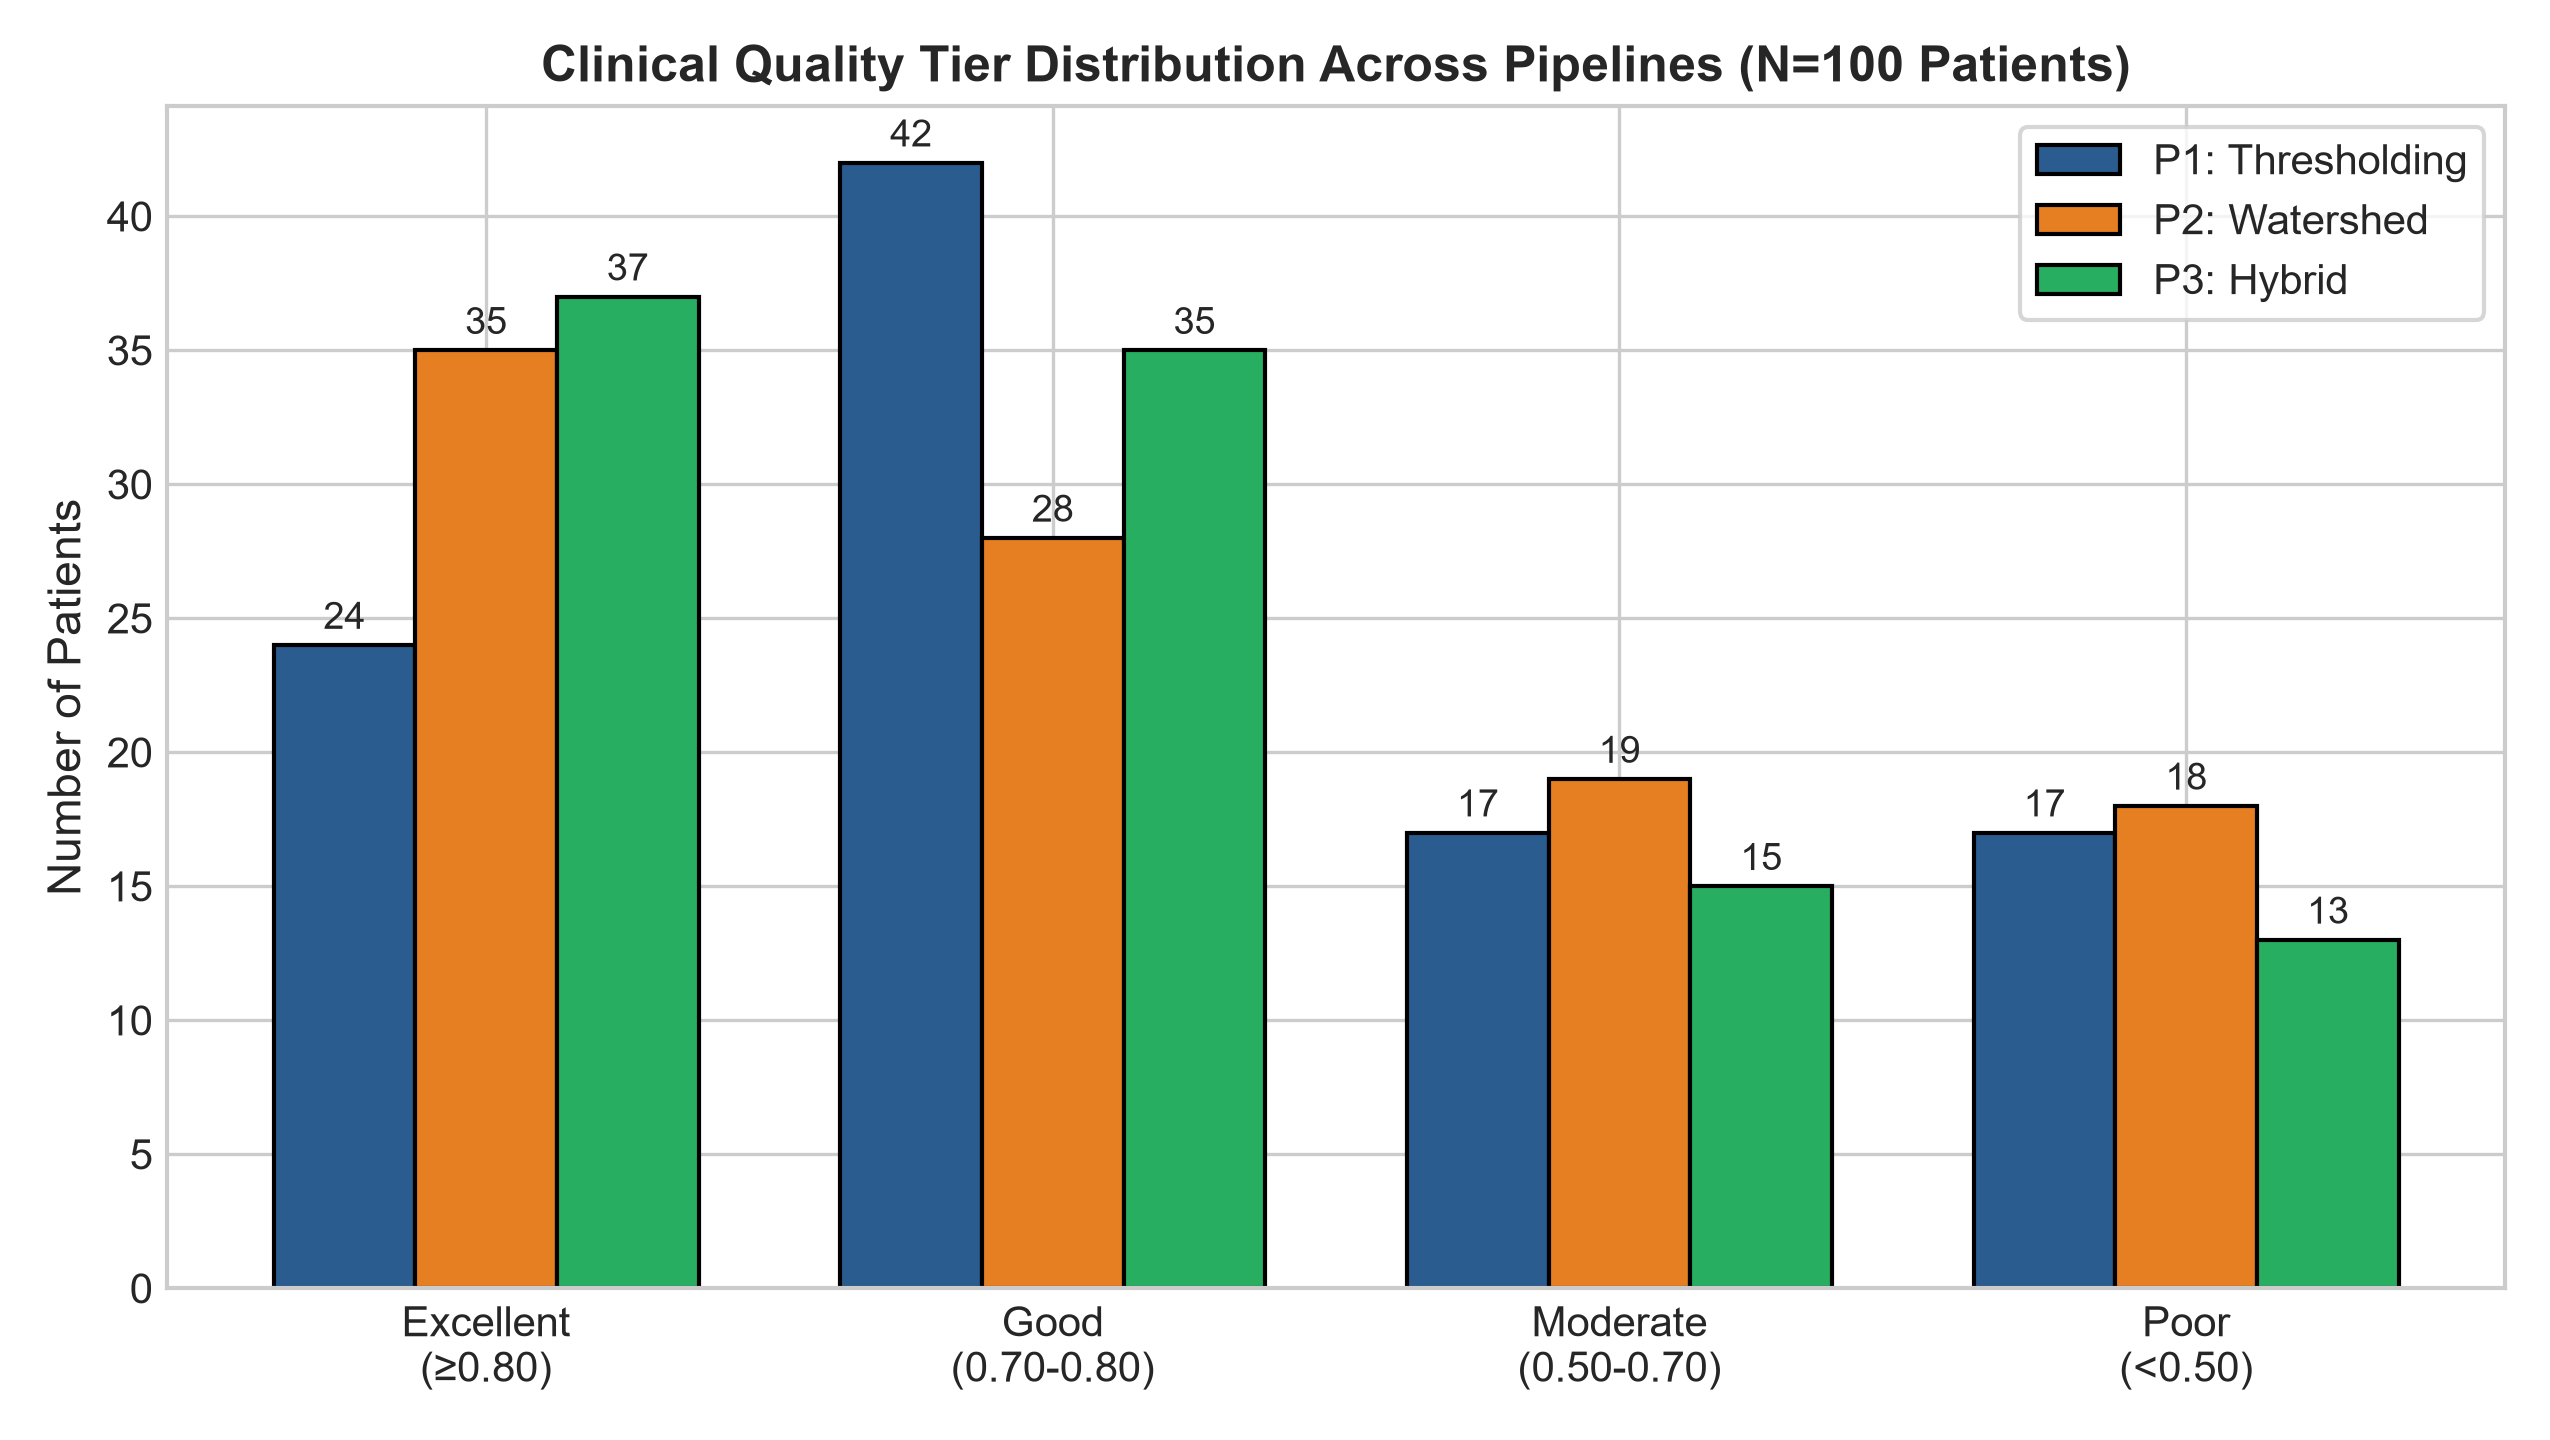
\includegraphics[width=\textwidth]{04_quality_tiers_bar.png}
    \caption{Quality Tier Distribution}
    \label{fig:tiers}
\end{subfigure}
\caption{Cohort segmentation distribution: (a) Head-to-head win tally across 100 patients. (b) Clinical quality tiers demonstrating Hybrid's concentration in Good and Excellent categories.}
\label{fig:distribution_charts}
\end{figure}

\begin{figure}[t]
\centering
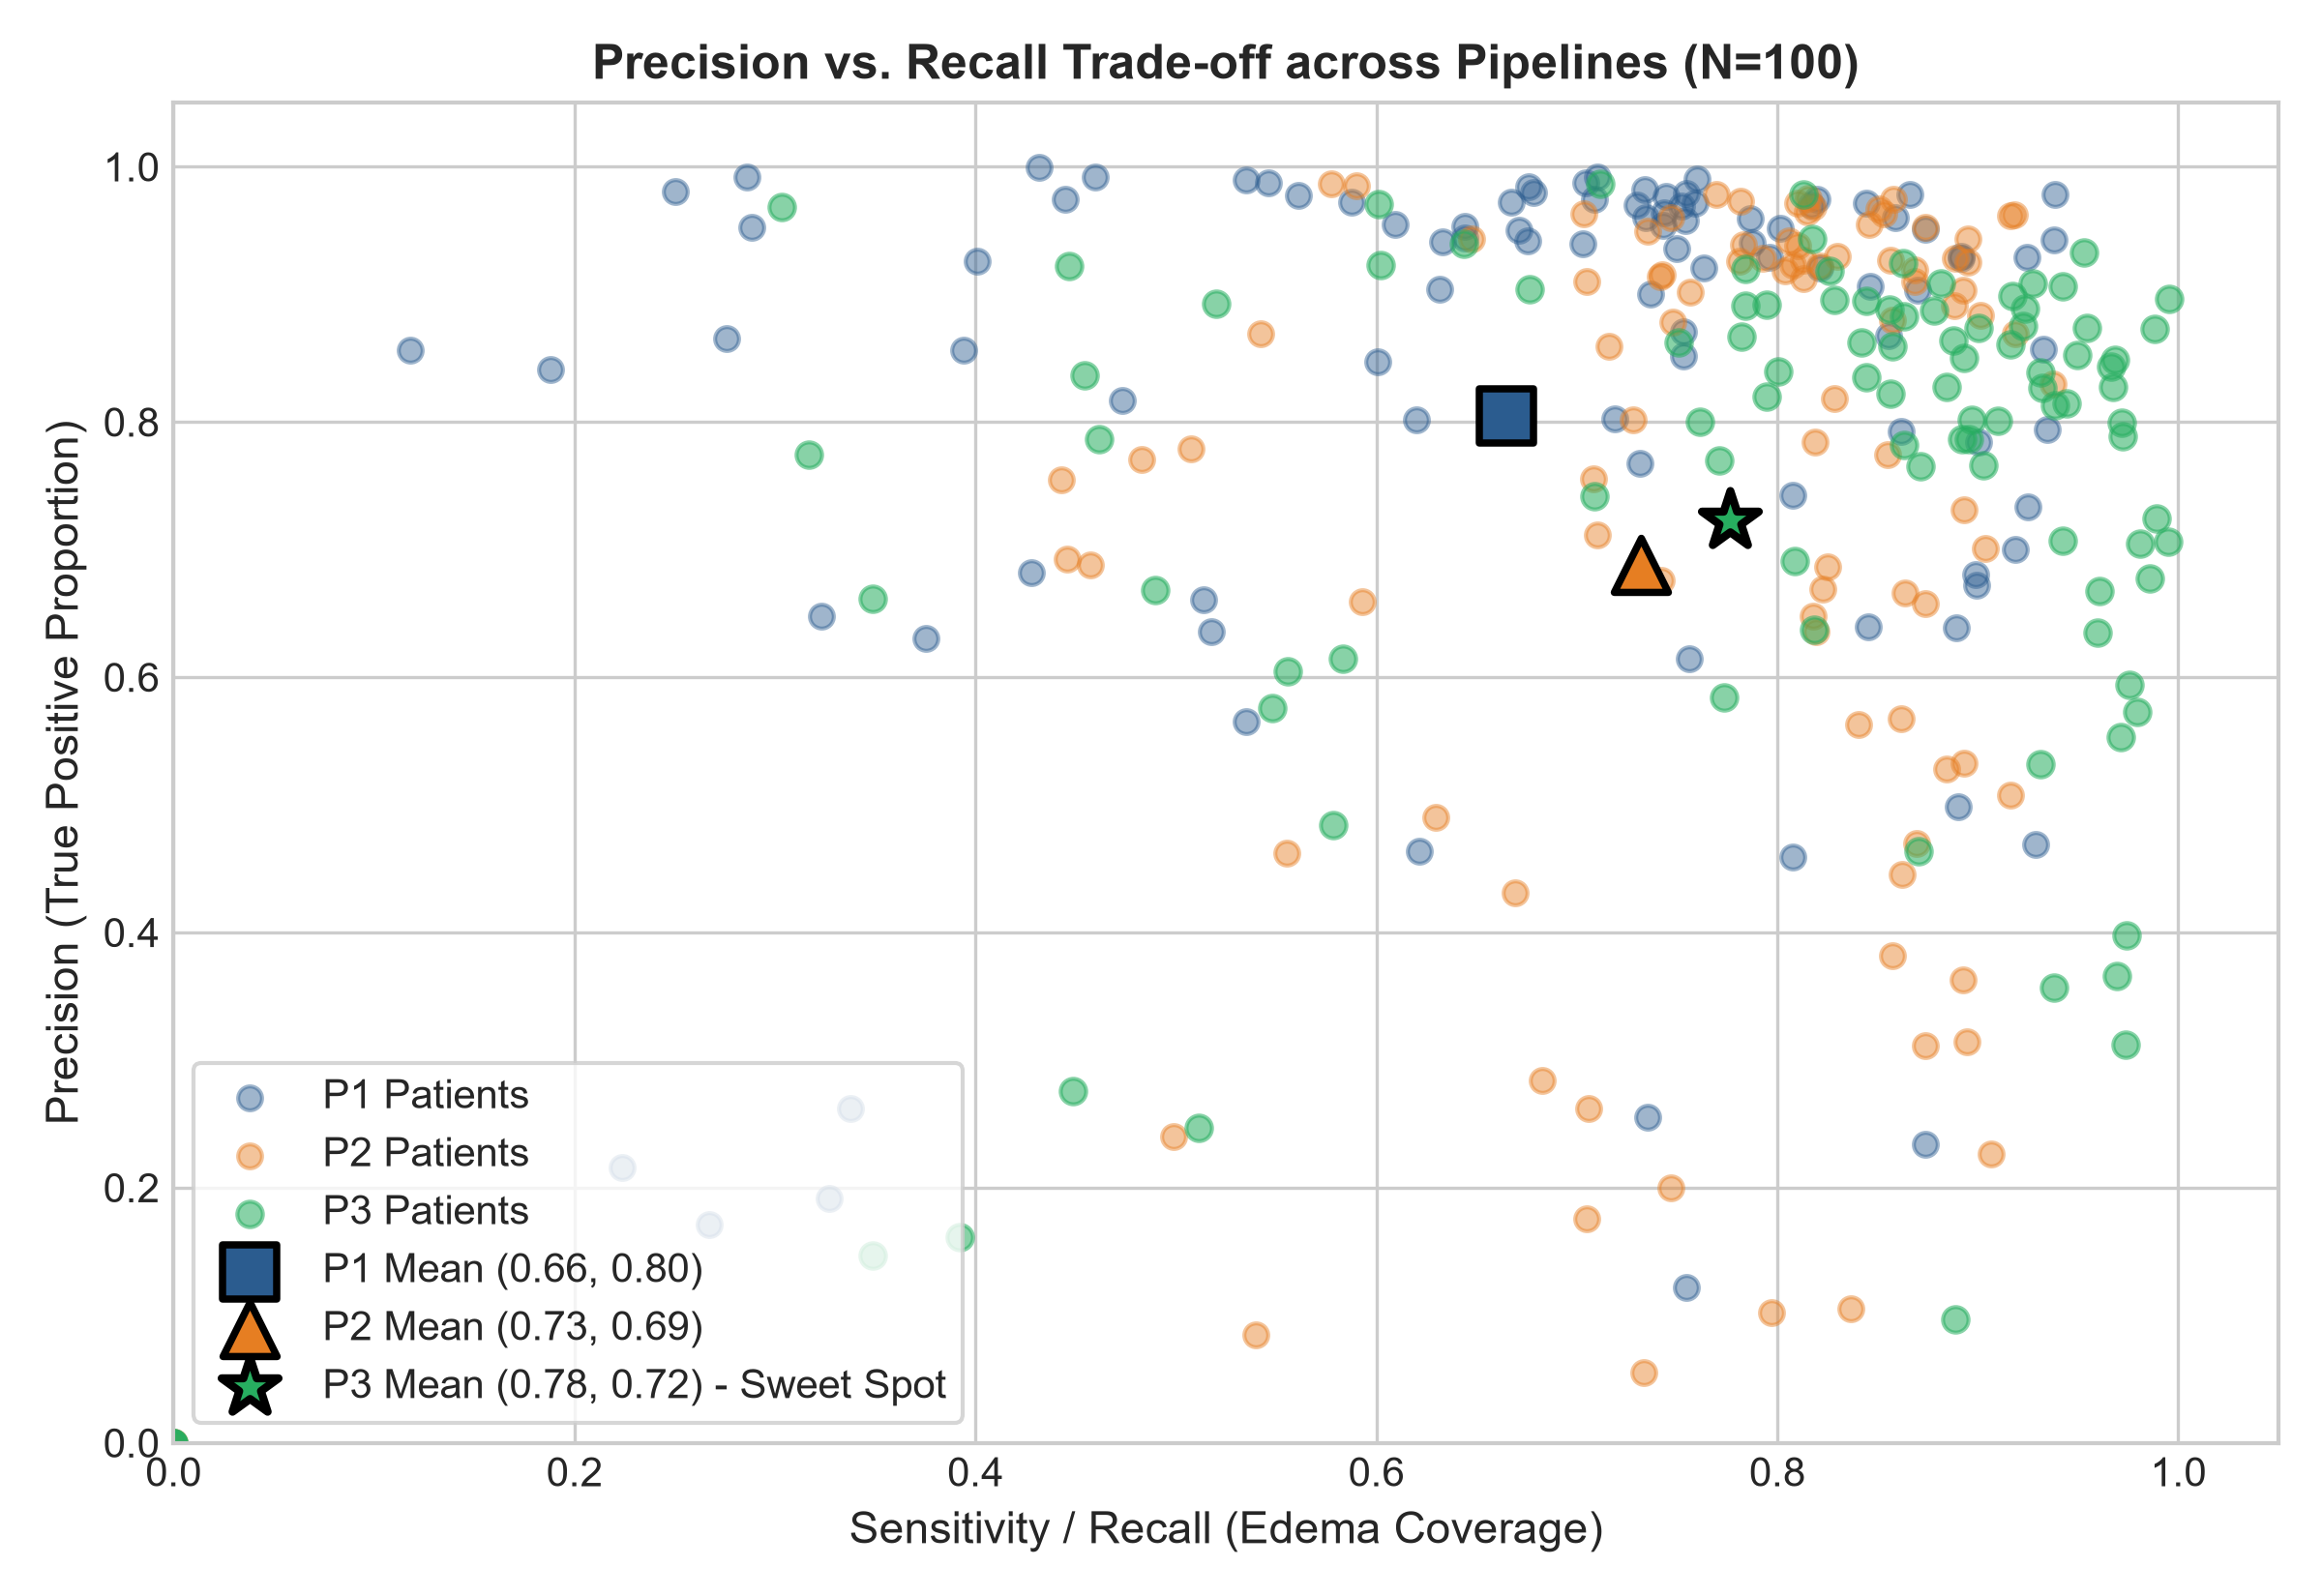
\includegraphics[width=0.85\columnwidth]{05_precision_recall_tradeoff.png}
\caption{Precision vs. Recall distribution for 100 patients. Centroids depict operating trade-offs: P1 favors precision, P2 favors recall, and P3 establishes the optimal Pareto-balanced sweet spot.}
\label{fig:pr_tradeoff}
\end{figure}

\subsection{Precision-Recall Dynamics and Failure Modes}
Fig.~\ref{fig:pr_tradeoff} illustrates the precision-recall trade-off across the cohort:
\begin{itemize}
    \item \textbf{Under-segmentation:} Dominates Pipeline 1 (49 cases), where diffuse edema fails rigid intensity cutoffs.
    \item \textbf{Over-segmentation:} Dominates Pipeline 2 (31 cases), where watershed floods across weak ventricular barriers.
    \item \textbf{Pareto Balance:} Hybrid reduces under-segmentation to 16 cases and curbs over-segmentation to 28 cases, establishing a superior centroid operating point ($0.78\text{ recall}, 0.72\text{ precision}$).
\end{itemize}

\subsection{Qualitative Visual Inspection}
Fig.~\ref{fig:mri_visuals} illustrates Patient BraTS20\_Training\_075, where Pipeline 3.0 achieves $DSC = \mathbf{0.9429}$ (IoU 0.8920, $HD_{95} = 4.0\text{ mm}$), tightly resolving non-convex tumor margins without spurious ventricular spillover.

\section{Discussion}
\subsection{Mathematical Mechanics of Hybrid Synergy}
Our results prove that Pipeline 3.0 is not a trivial boolean union ($M_{\text{P1}} \cup M_{\text{P2}}$), which would compound false positives. Instead, it functions as an \textbf{asymmetric mutual constraint}:
\begin{enumerate}
    \item \textbf{Topological Seeding:} Thresholding provides verified core seeds ($M_{\text{core}}$), eliminating watershed's vulnerability to over-segmentation from spurious local minima.
    \item \textbf{Geodesic Search Confinement:} Watershed flooding is restricted to a narrow geodesic band $\Omega_{\text{allowed}}$, preventing leakage into ventricles or contralateral tissue.
    \item \textbf{Edge Regularization:} The 3D Gaussian gradient guides final boundaries along authentic tissue transition ridges, smoothing jagged threshold edges.
\end{enumerate}

\subsection{Academic Validity and Negative Edge Cases}
In 29\% of cases, Pipeline 1.0 (Thresholding) outperformed Hybrid. In dense, focal lesions with negligible edema (e.g., Patient 098, $DSC = 0.9581$), the dilation envelope of Pipeline 3 introduced slight boundary padding, reducing precision. Conversely, in diffuse infiltrative lesions (e.g., Patient 066, where Hybrid achieved $DSC = 0.9079$ vs. 0.7490 for P1), hybridization was essential.

\subsection{Computational Efficiency}
All pipelines run deterministically on standard CPUs without GPU hardware. Full 3D execution per volume requires $\approx 18\text{ s}$ for Pipeline 1.0, $\approx 24\text{ s}$ for Pipeline 2.0, and $\approx 26\text{ s}$ for Pipeline 3.0, making classical hybrid methods well suited for resource-constrained clinical settings.

\section{Conclusion}
This study evaluated classical DIP paradigms for multi-modal brain tumor segmentation across 100 BraTS 2020 patients. By coupling intensity-derived topological priors with geodesic-constrained gradient flooding, Pipeline 3.0 (Hybrid) achieved a median Dice score of 0.8215 and a 42\% win rate, resolving thresholding under-segmentation while preventing watershed leakage. The results confirm that classical image processing, when anatomically and mathematically bounded, delivers robust, explainable, and clinically meaningful segmentation without deep learning complexity.

\begin{thebibliography}{00}
\bibitem{menze2015brats} B. H. Menze \textit{et al.}, ``The Multimodal Brain Tumor Image Segmentation Benchmark (BRATS),'' \textit{IEEE Trans. Med. Imag.}, vol. 34, no. 10, pp. 1993--2024, Oct. 2015.
\bibitem{bakas2017advancing} S. Bakas \textit{et al.}, ``Advancing The Cancer Genome Atlas glioma analysis with pre-computed calculations and computerized labels,'' \textit{Sci. Data}, vol. 4, art. no. 170117, Sep. 2017.
\bibitem{vincent1991watersheds} L. Vincent and P. Soille, ``Watersheds in digital spaces: an efficient algorithm based on immersion simulations,'' \textit{IEEE Trans. Pattern Anal. Mach. Intell.}, vol. 13, no. 6, pp. 583--598, Jun. 1991.
\bibitem{otsu1979threshold} N. Otsu, ``A threshold selection method from gray-level histograms,'' \textit{IEEE Trans. Syst., Man, Cybern.}, vol. 9, no. 1, pp. 62--66, Jan. 1979.
\bibitem{tomasi1998bilateral} C. Tomasi and R. Manduchi, ``Bilateral filtering for gray and color images,'' in \textit{Proc. 6th IEEE Int. Conf. Comput. Vis. (ICCV)}, 1998, pp. 839--846.
\bibitem{gonzalez2018dip} R. C. Gonzalez and R. E. Woods, \textit{Digital Image Processing}, 4th ed., Pearson, 2018.
\bibitem{akiba2019optuna} T. Akiba \textit{et al.}, ``Optuna: A next-generation hyperparameter optimization framework,'' in \textit{Proc. 25th ACM SIGKDD (KDD)}, 2019, pp. 2623--2631.
\end{thebibliography}

\end{document}
